\documentclass[a4paper,11pt]{book}

% Essential packages
\usepackage[utf8]{inputenc} % UTF-8 encoding
\usepackage[T1]{fontenc}    % Font encoding
\usepackage[english]{babel} % English language
\usepackage{graphicx}       % For including images
\usepackage[version=4]{mhchem} % chemical package
\usepackage{amsmath, amssymb} % Advanced math symbols
\usepackage{hyperref}       % For clickable links
\usepackage{geometry}       % For custom margins
\usepackage{setspace}       % For line spacing
\usepackage{fancyhdr}       % For headers and footers
\usepackage{biblatex}       % For bibliography management
\usepackage{listings}
\usepackage{booktabs}
\usepackage{caption}   % Per personalizzare le didascalie
\usepackage{subcaption} % Per immagini affiancate
\usepackage{array}
\usepackage{colortbl}
\usepackage{xcolor} % Per definire colori personalizzati

\lstset{
    basicstyle=\ttfamily\small,  % Tipo di carattere (monospace)
    keywordstyle=\bfseries,      % Parole chiave in grassetto
    commentstyle=\itshape,       % Commenti in corsivo
    columns=fullflexible,        % Allineamento corretto
    frame=single,                % Bordo intorno al codice
    breaklines=true,             % Andare a capo automaticamente
    captionpos=b                 % Posizione della caption (bottom)
}
% Set margins
\geometry{
    a4paper,
    top=3cm,
    bottom=3cm,
    left=3cm,
    right=3cm,
}

% Line spacing
\onehalfspacing

% Header and footer setup
\pagestyle{fancy}
\fancyhf{}
\fancyhead[L]{\leftmark}
\fancyfoot[C]{\thepage}

% Load bibliography
\addbibresource{bibliography.bib}

\begin{document}

%%%%%%%%%%%%%%%%%%%%%%%%%%%%%%%%%%%%%%%%%%%%%%%%%%%%%%%%%%%%%%%%%

%%%%%%%%%%%%%%%%%%%%%%%%%%%%%%%%%%%%%%%%%%%%%%%%%%%%%%%%%%%%%%%%%

\chapter*{Results with BCS theory}
Now that we can solve Eqs.~\ref{eq:MB-real_cond} and~\ref{eq:MB-imag_cond} let's see the results for some 
different materials and various temperatures. In particular i have tested Nb, Pb and Al.

For different materials we need the experimental values of thecritical temperature $T_c$, under which they become superconductors, and the zero temperature value of the enrgy gap $\Delta_0$.
Actually for $\Delta_0$ we extract the value from the BCS relation
\begin{equation}
    \frac{2\Delta_0}{K_BT_c} = \alpha,
\end{equation}
where $\alpha$ is $\sim 3.53$ for weak-coupling materials, that is the limit where BCS theory and MB formulas
holds, and is greater for strong-coupling materials such as Nb and Pb. In Tab.~\ref{tab:T_c} below the $T_c$ and $\alpha$ values are showed.


\begin{table}[]
\centering
\caption{Superconducting materials experimental parameters.}
\begin{tabular}{@{}lll@{}}
\toprule
Material & $T_c$(K) & $\alpha$ \\ \midrule
Nb       & 9.3      & 3.65     \\
Pb       & 7.2      & 3.95     \\
Al       & 1.2      & 3.53     \\ \bottomrule
\end{tabular}
\label{tab:T_c}
\end{table}

Since $\Delta = \Delta (T)$ is a function of the temperature and is zero at $T \geq T_c$ i have extrapolate it in the BCS approximation as
\begin{equation}
    \Delta = \Delta_0~\tanh \left(e^{\gamma}\sqrt{\frac{8}{7\xi (3)}}~\sqrt{\frac{T_c}{T} - 1} \right) \simeq \Delta_0~\tanh \left(1.74~\sqrt{\frac{T_c}{T} - 1}\right).
    \label{eq:BCS_gap_approx}
\end{equation}

In the following we see some test for Nb, Pb and Al at different temperatures. In Fig.~\ref{fig:figura_cond_comparison} i compared the real and imaginary conductivity for 
Nb, Pb and Al at $T=0.8T_c$. In Fig.~\ref{fig:figura_completa_Nb} we see conductivity of Nb for different temperatures. The last Fig.~\ref{fig:figura_completa_Nb_norm} i have plotted the conductivity of
Niobium with the energy scale normalized by $2\Delta_0$ to check if the real part of $\sigma / \sigma_n$ correctly 
drops down at $\hbar \omega = 2\Delta_0$ when $T=0$, and if increasing $T$ the gap moves to lower energies/frequencies. 
\begin{figure}
    \centering
    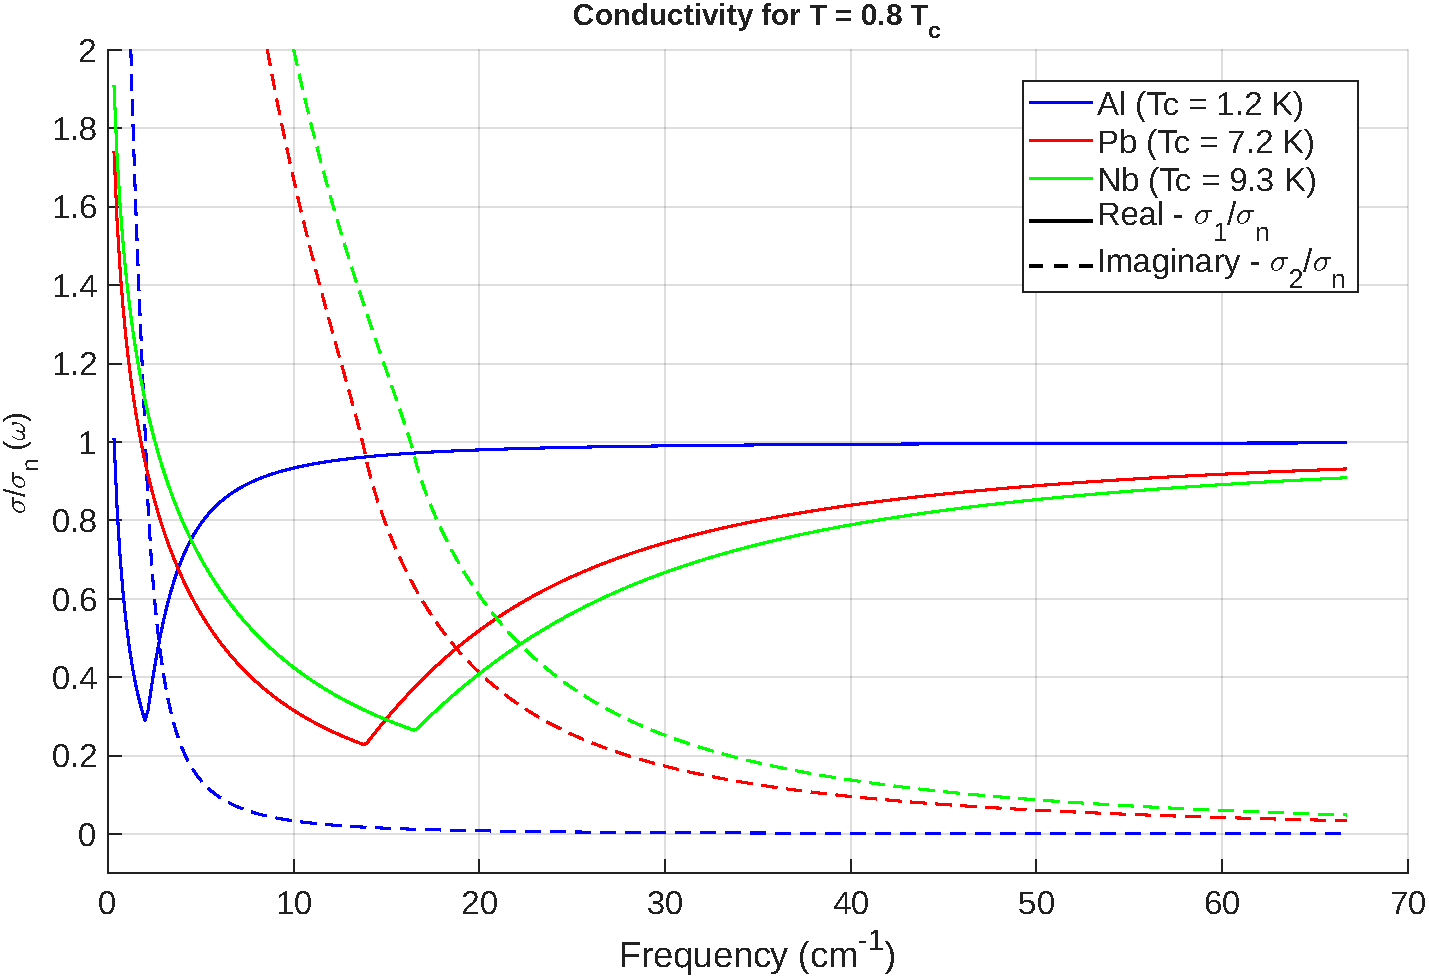
\includegraphics[width=0.8\textwidth]{../Immages/BCS_Comparison_0.8Tc.pdf}
    \caption{Complex conductivity for different materials.}
     \label{fig:figura_cond_comparison}
\end{figure}

\begin{figure}[!h]
    \centering
    % Sotto-figura di SINISTRA
    \begin{subfigure}[b]{0.49\textwidth}
        \centering
        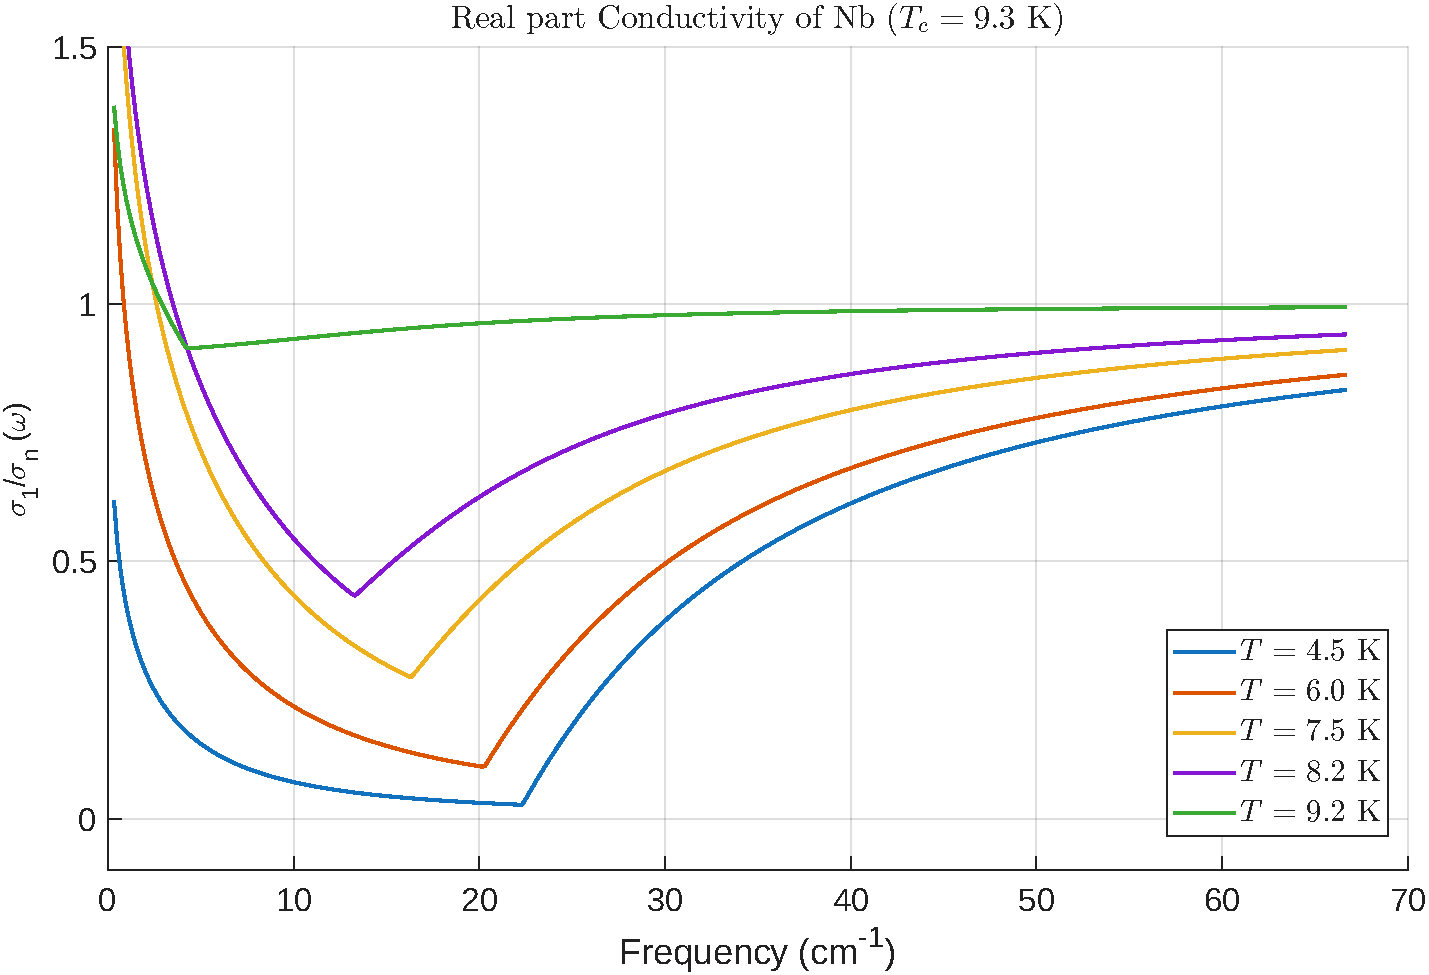
\includegraphics[width=\textwidth]{../Immages/BCS_Nb_real_cond_diffT_conv_units.pdf}
        %\caption{Didascalia dell'immagine a sinistra.}
        \label{fig:sinistra_Nb}
    \end{subfigure}
   \hfill
    % Sotto-figura di DESTRA
    \begin{subfigure}[b]{0.49\textwidth}
        \centering
        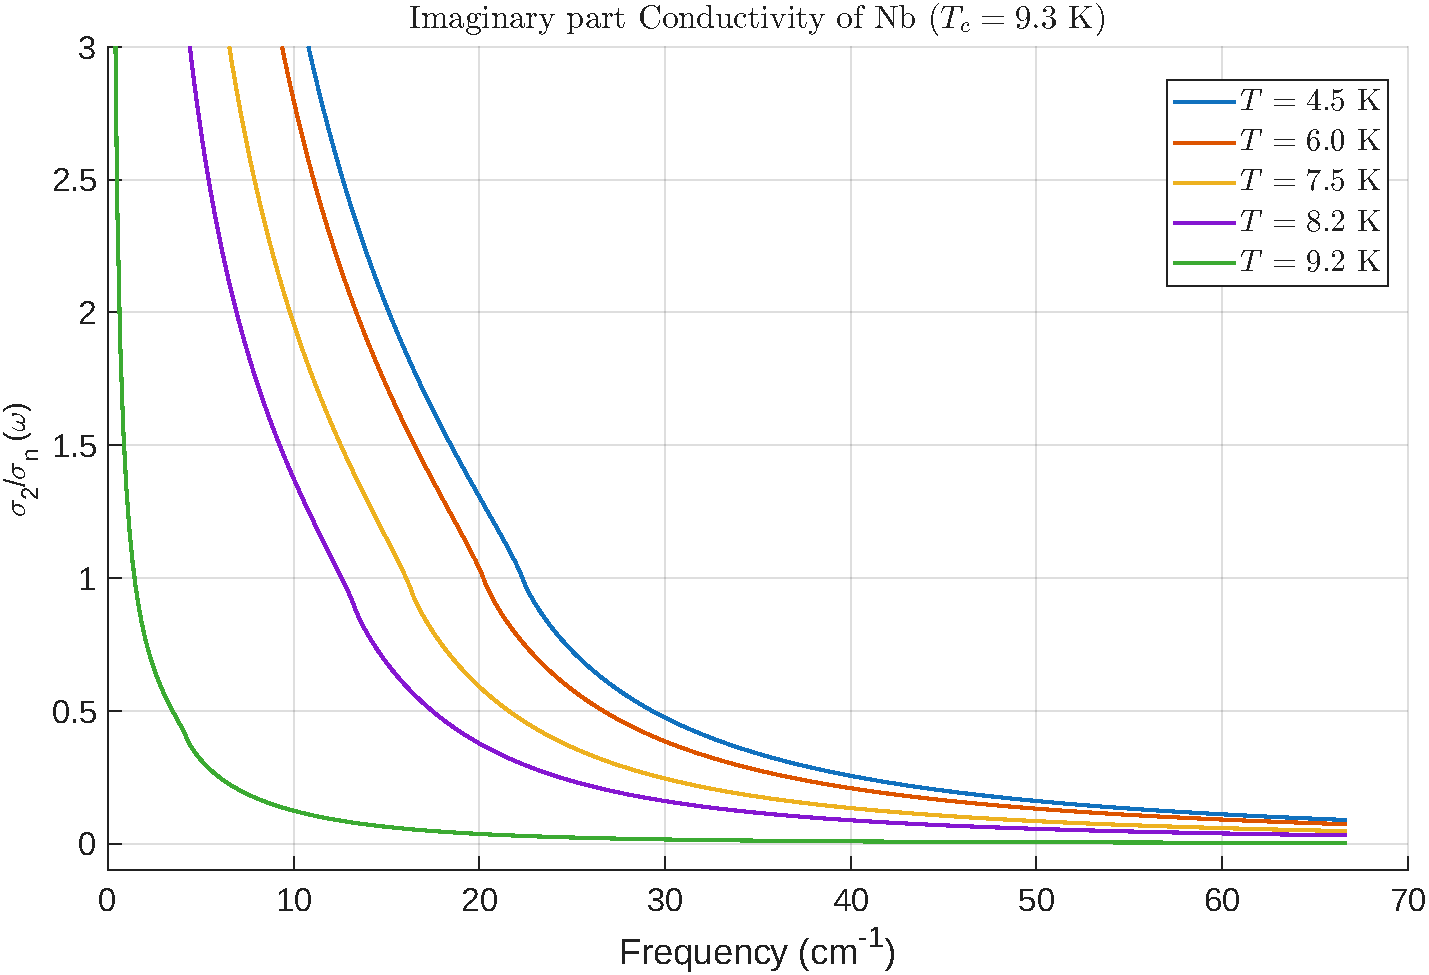
\includegraphics[width=\textwidth]{../Immages/BCS_Nb_imm_cond_diffT_conv_units.pdf}
        %\caption{Didascalia dell'immagine a destra.}
        \label{fig:destra_Nb}
    \end{subfigure}
    
    % Didascalia e Label GENERALI di tutta la figura
    \caption{Real (sx) and imaginary (dx) conductivity for Nb.}
    \label{fig:figura_completa_Nb}
\end{figure}


\begin{figure}[!h]
    \centering
    % Sotto-figura di SINISTRA
    \begin{subfigure}[b]{0.49\textwidth}
        \centering
        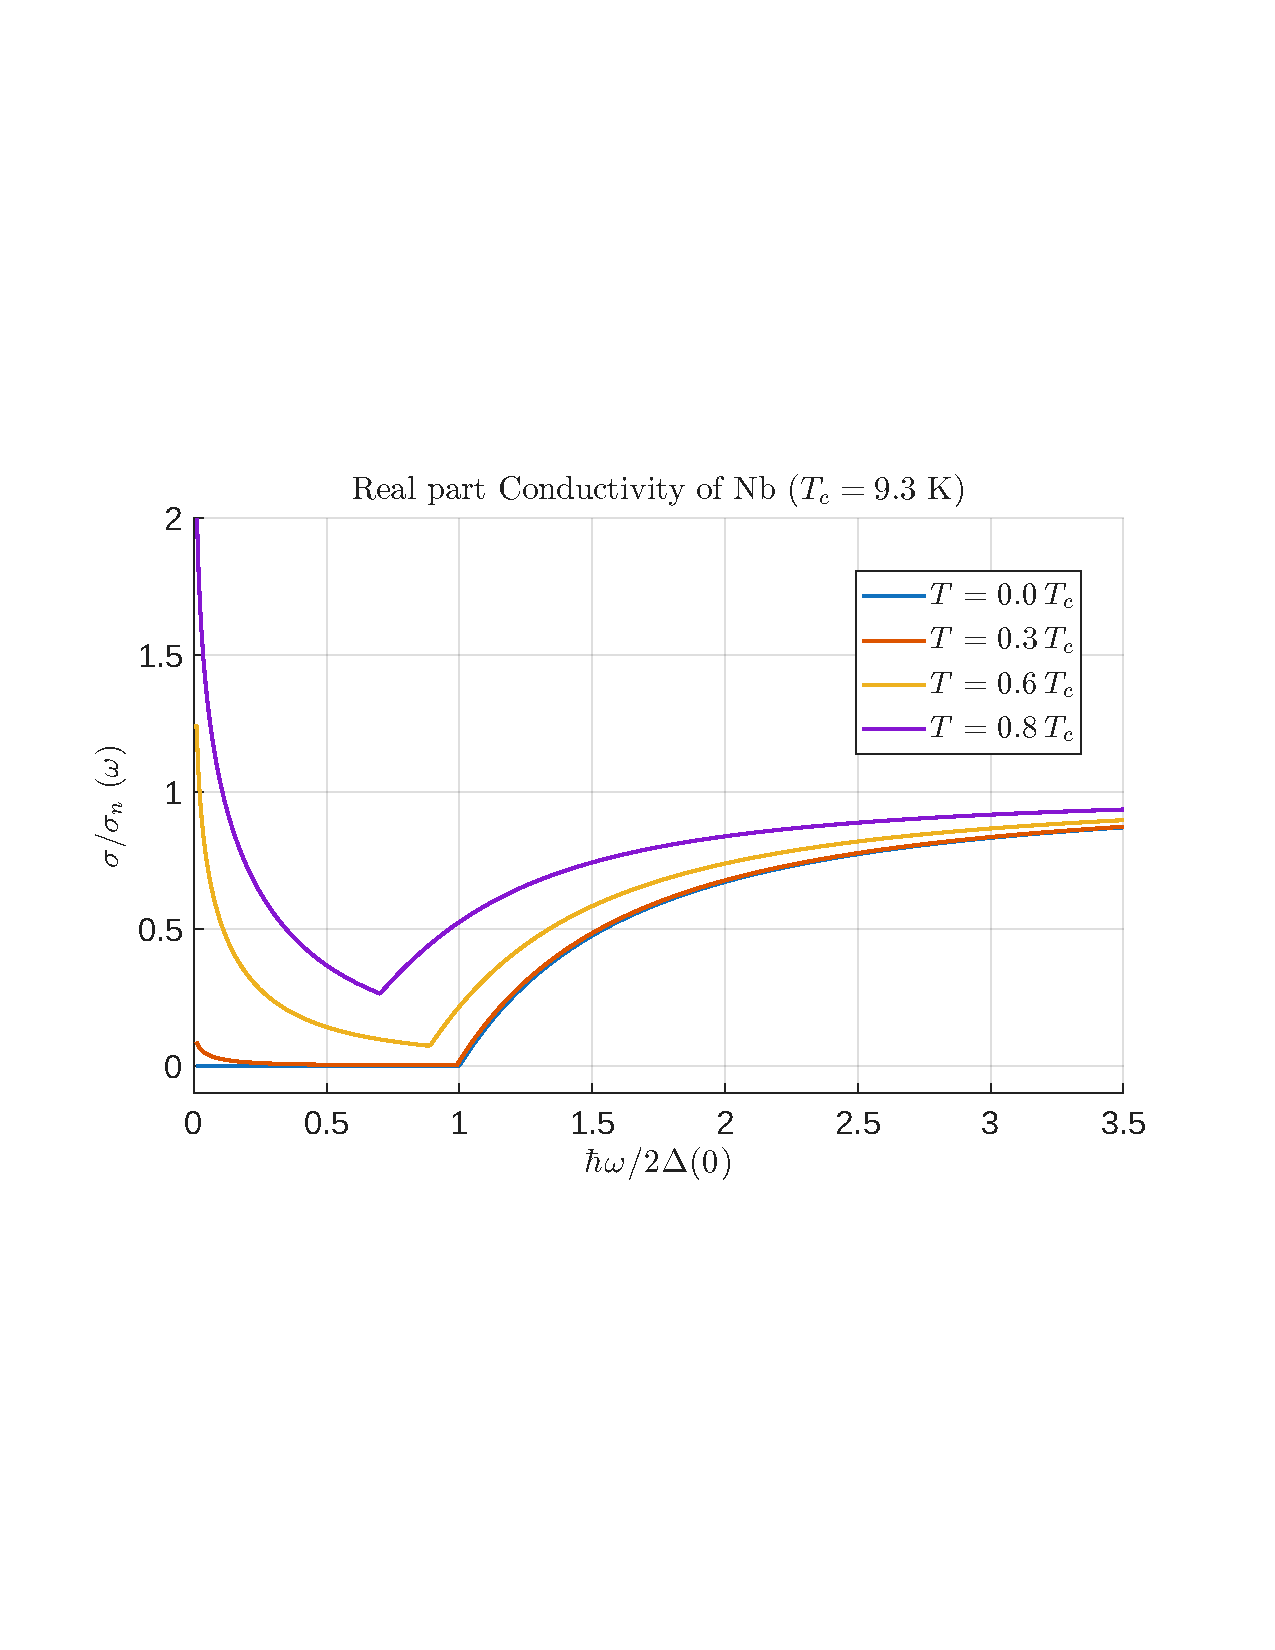
\includegraphics[width=\textwidth]{../Immages/BCS_Nb_real_cond_diffT.pdf}
        %\caption{Didascalia dell'immagine a sinistra.}
        \label{fig:sinistra_Nb_norm}
    \end{subfigure}
    \hfill
    % Sotto-figura di DESTRA
    \begin{subfigure}[b]{0.49\textwidth}
        \centering
        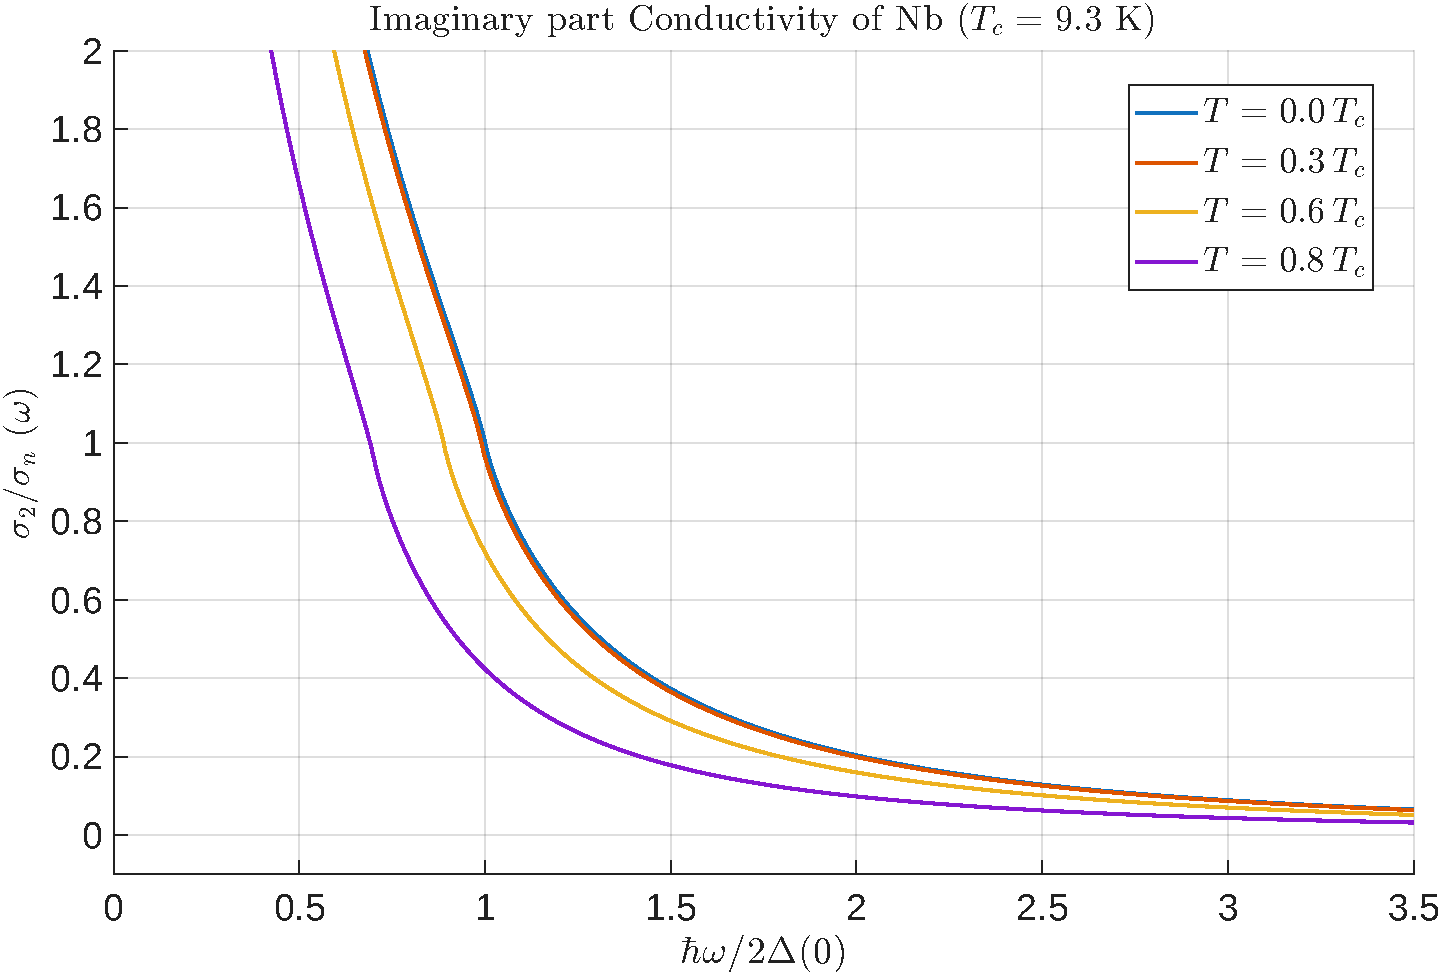
\includegraphics[width=\textwidth]{../Immages/BCS_Nb_imm_cond_diffT.pdf}
        %\caption{Didascalia dell'immagine a destra.}
        \label{fig:destra_Nb_norm}
    \end{subfigure}
    
    % Didascalia e Label GENERALI di tutta la figura
    \caption{Real (sx) and imaginary (dx) conductivity for Nb in normalized units, to check the gap corresponds at $T=0$.}
    \label{fig:figura_completa_Nb_norm}
\end{figure}

\section*{Comparison with experiments}

To evaluate the performances of the code that i've written, i compare the numerical solutions
with experimental data of Nb. To extract the data points from the figure i have used the online tool \texttt{WebPlotDigitizer}.
The results are showed in the Fig.\ref{fig:figura_completa_Nb_fit} below with $T_c=8.3$~K and $\alpha=4.1$.
\begin{figure}[!h]
    \centering
    % Sotto-figura di SINISTRA
    \begin{subfigure}[b]{0.6\textwidth}
        \centering
        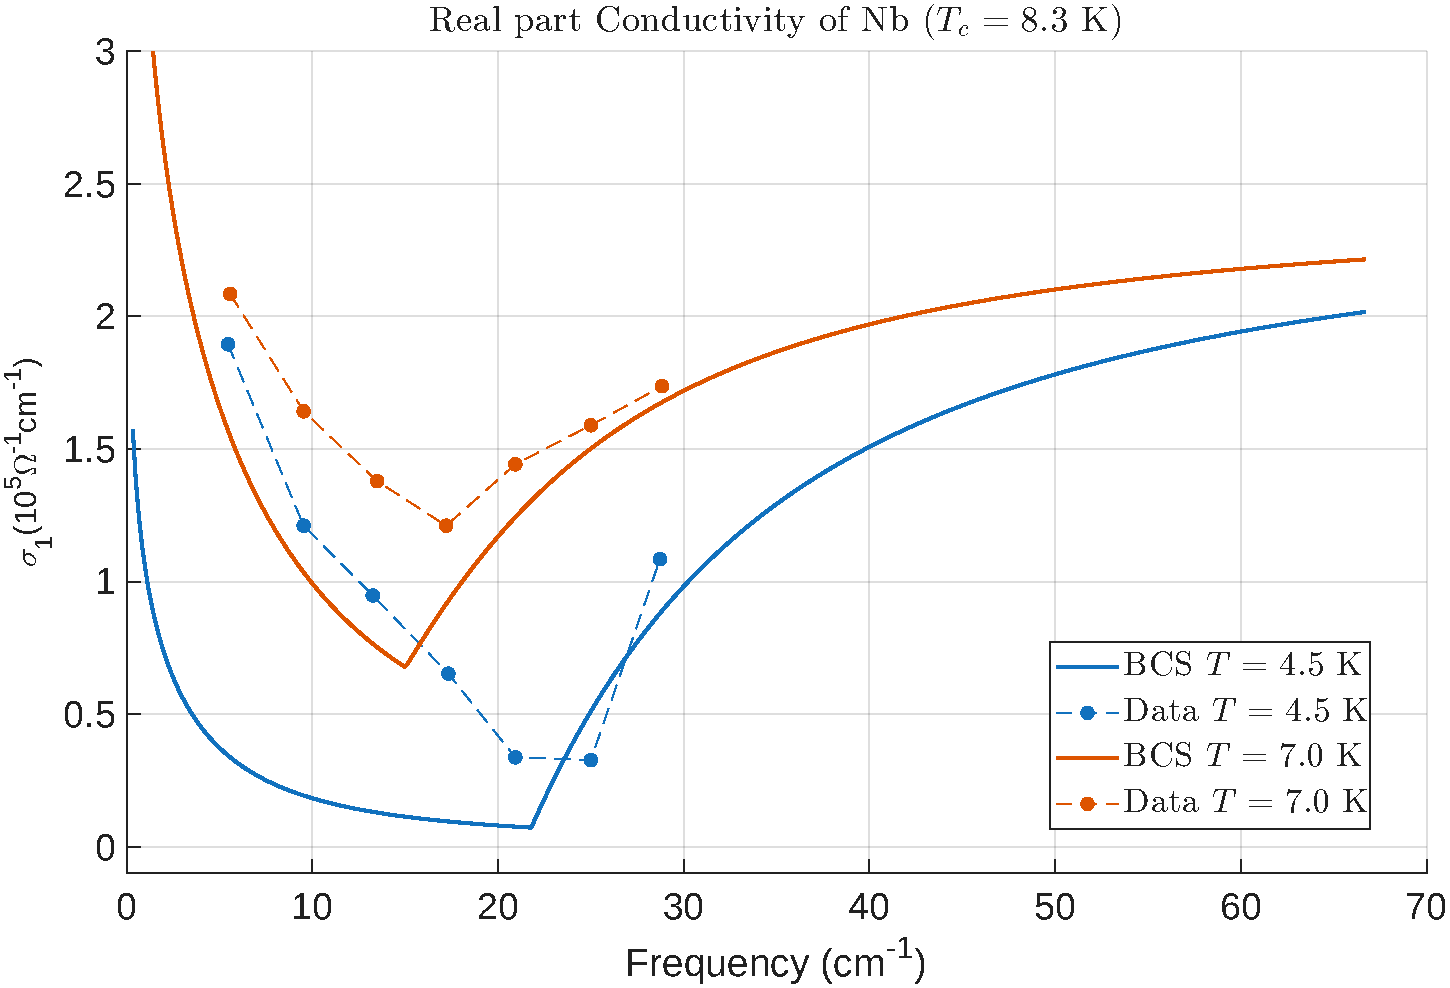
\includegraphics[width=\textwidth]{../Immages/BCS_Nb_real_cond_diffT_conv_units_fitexp.pdf}
        %\caption{Didascalia dell'immagine a sinistra.}
        \label{fig:sinistra_Nb_fit}
    \end{subfigure}

    % Sotto-figura di DESTRA
    \begin{subfigure}[b]{0.6\textwidth}
        \centering
        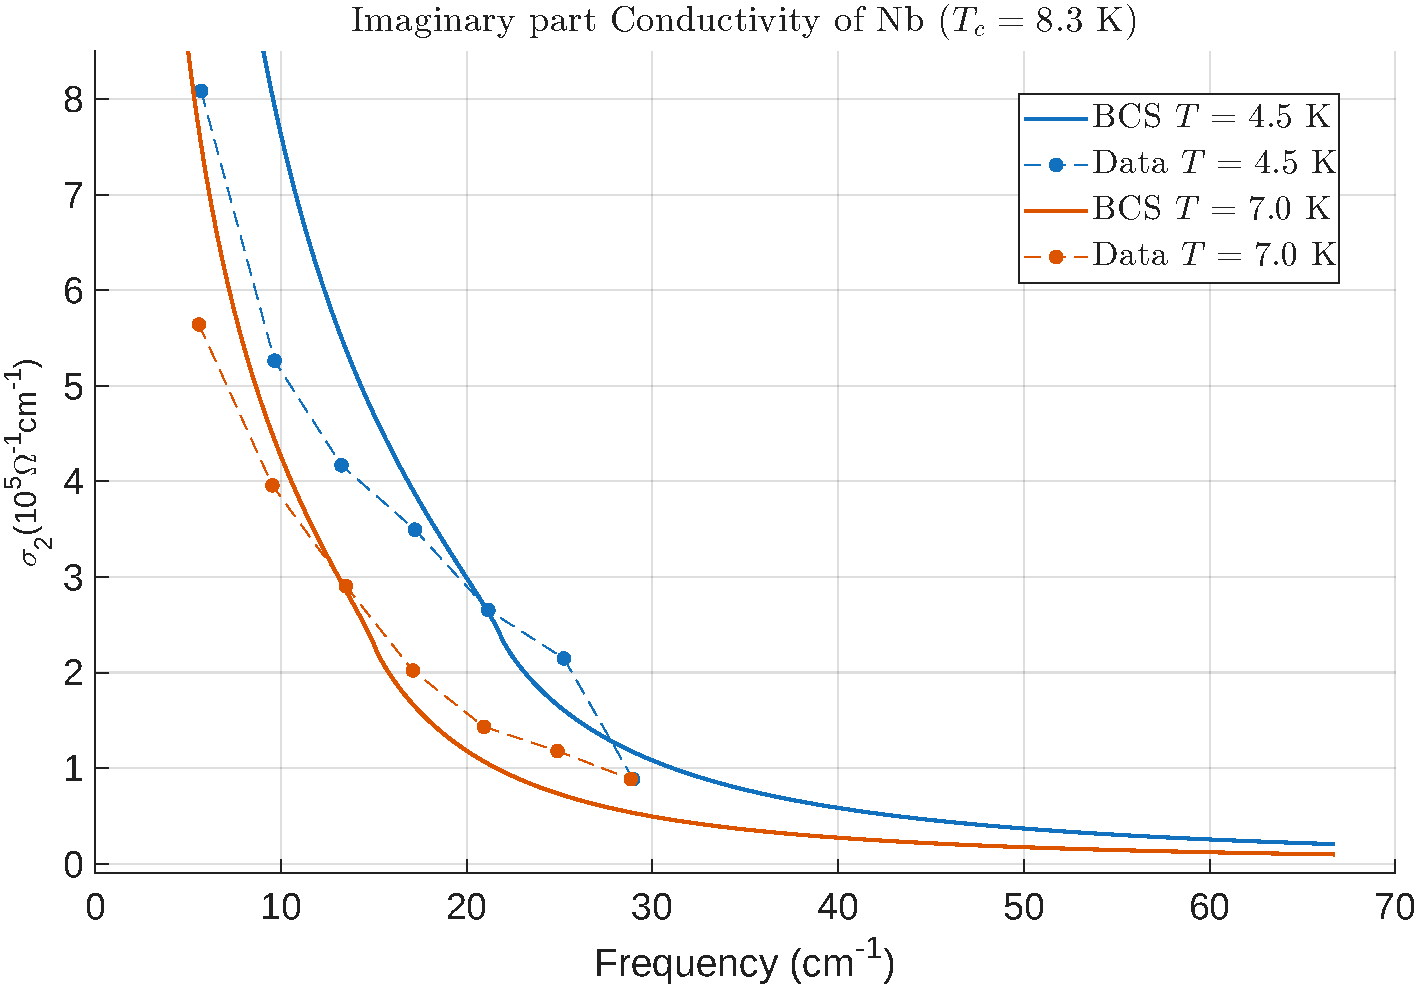
\includegraphics[width=\textwidth]{../Immages/BCS_Nb_imm_cond_diffT_conv_units_fitexp.pdf}
        %\caption{Didascalia dell'immagine a destra.}
        \label{fig:destra_Nb_fit}
    \end{subfigure}
    
    % Didascalia e Label GENERALI di tutta la figura
    \caption{Real (sx) and imaginary (dx) conductivity for Nb compared with experimental data.}
\label{fig:figura_completa_Nb_fit}
\end{figure}
We can see that the BCS understimates the value of the real conductivity $\sigma_1$, expecially for lower $T$, but we espected this for Niobium because is a strong-coupling
superconducting material while BCS is a weak-coupling theory ($\alpha = 3.65$). 

Another comparison that needs to be done is the one between the values of $\Delta$ at different temperatures extracted 
by the experimental data of conductivity, and the BCS mean field approximation used for the gap function in Eq.~\ref{eq:BCS_gap_approx}. The value of $2\Delta(T)$
is given by the frequency that corresponds to the minimum of the $\sigma_1$ at given temperature.
This is showed in Fig.~\ref{fig:Gap_comparison}. Furthermore in Fig.~\ref{fig:Gap_comparison} i have plotted the frequency at the minimum of $\sigma_1$ obtained
from the numerical solution of Mattis-Bardeen as a counter check for the code.

\begin{figure}[!h]
    \centering
    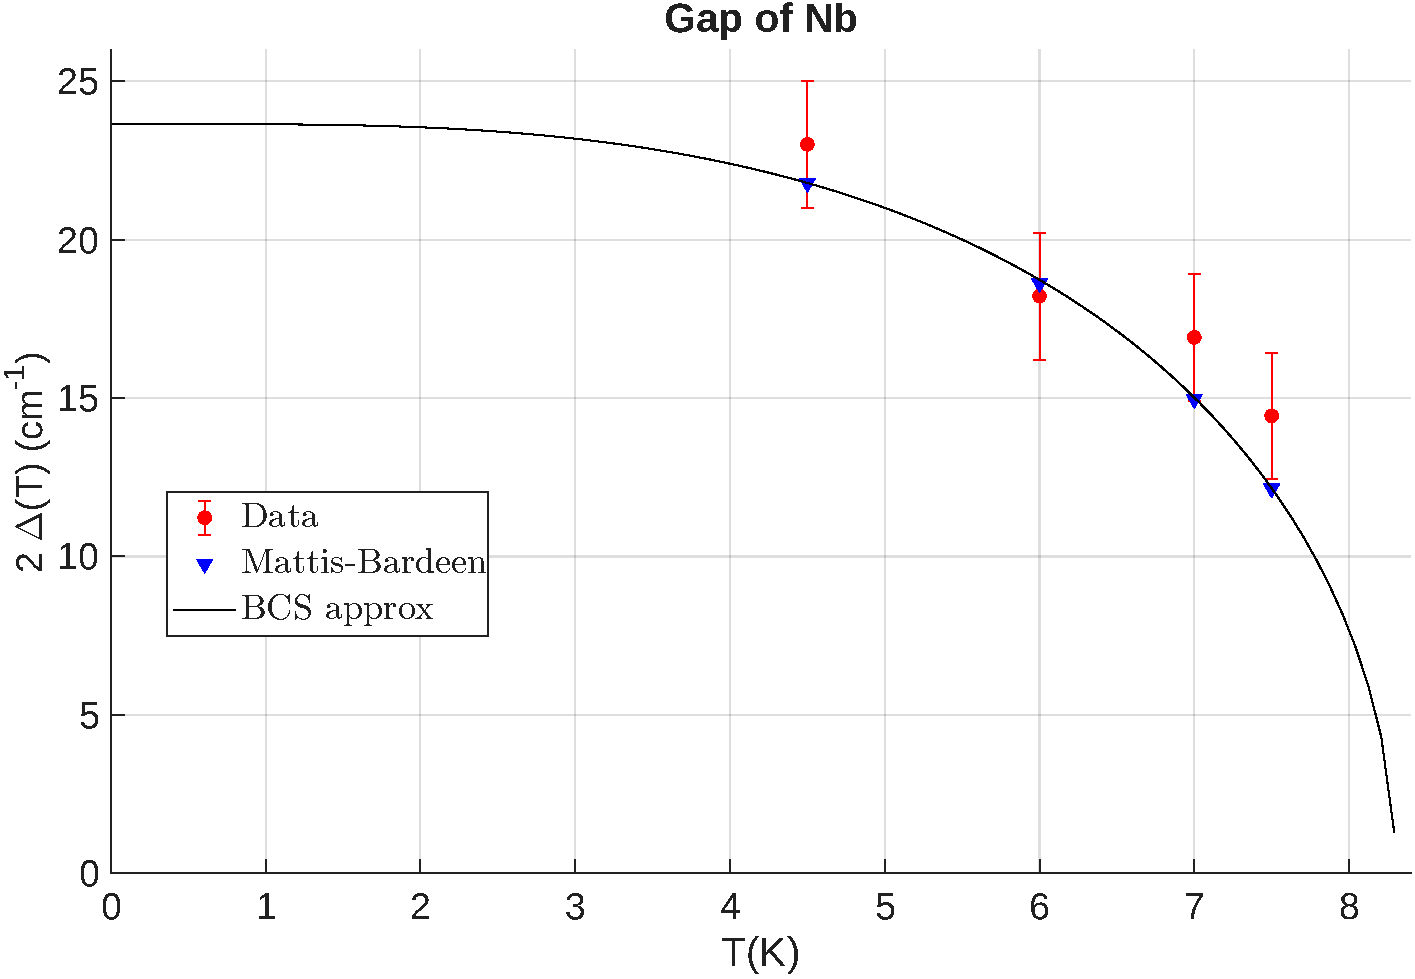
\includegraphics[width=0.7\textwidth]{../Immages/BCS_Gap_MB_vs_T_fitexp.pdf}
    \caption{Comparison between BCS approximation of $\Delta(T)$ and the values of $\Delta$ extracted by the data. Errorbars are $2~\text{cm}^{-1}$ from the paper [ref].}
\label{fig:Gap_comparison}
\end{figure}

\end{document}